\documentclass{article}
\usepackage[margin=1in]{geometry}
\usepackage{xcolor}
\usepackage{adjustbox}
\usepackage{verbatim}
\definecolor{shadecolor}{rgb}{.9, .9, .9}
\usepackage{tcolorbox}
\usepackage[colorlinks = true,
            linkcolor = blue,
            urlcolor  = blue,
            citecolor = blue,
            anchorcolor = blue]{hyperref}

\newenvironment{code}%
   {\par\noindent\adjustbox{margin=1ex,bgcolor=shadecolor,margin=0ex \medskipamount}\bgroup\minipage\linewidth\verbatim}%
   {\endverbatim\endminipage\egroup}


%\DeclareUrlCommand{\burl}{\def\UrlFont{\ttfamily\color{blue}}}

\newcommand{\burl}[3][blue]{\href{#1}{\color{#2}{#3}}}%

\title{Conducting experiments on Mechanical Turk via {\em mturkutils}}
\author{Florian Jaeger with help from Linda Liu, Zach Burchill, Wednesday Bushong, and Xin Xie}

\begin{document}

\maketitle

\tableofcontents

\section{Overview}

Make sure you have completed the tutorial on {\em Setting up Mechanical Turk and boto(3)}. Now that you are familiar with boto(3) and the mturkutils, it is time to get started on your own experiment. This tutorial walks you through how to sandbox your experiment on MTurk's sandbox, how to upload the (thoroughly tested) HIT to MTurk, and how to collect your data once all assignments for the HIT have been completed. This tutorial does {\em not} describe how to program your own experiment.


\section{Develop and debug your experiment locally}

After you have completed the HTML (and potentially Javascript or other) programming necessary for your experiment, the first recommended step is to debug the experiment locally on your computer. In many cases, you will not even need to install a local webserver on your computer. If your experiment does not record speech, video, or alike but only {\em presents} audio, video, or other stimuli then you likely will be able to simply open your HTML file on your computer in a browser. This allows you to go through your experiment and debug it. \textbf{Only after you have completed local debugging of your experiment, is it time to test whether your experiment also works on MTurk.}



\section{Sandbox a HIT}

The first step following completed developing and debugging is to {\em sandbox} your experiment. The MTurk sandbox provides an online testing environment that works like the real MTurk while avoiding that you have to pay for the HIT. You can host a HIT on the MTurk sandbox and then you or other team members can take that HIT in order to debug it. This will also be the first step in your debugging process at which you can test whether the data that you obtain from a completed HIT assignment is in the intended format.

You can walk through the steps described next using your own experiment, or using the short mock experiment contained in this tutorial. This mock experiment is hosted on the HLP Lab web server, and you won't have to modify it at all.

\begin{itemize}

   \item Using your favorite text editor, check out the contents of example-HIT.yaml in the hits/ folder. This is a YAML configuration file. {\bf YAML configuration files specify the basic information for MTurk HITs} that {\em mturkutils} will use ot upload your HIT(s). This includes the HIT description, the payment, the url that specifies where the experiment is hosted, and more (we'll cover configuration files in a more detail in Section \ref{sec:batchify}). 
   
   \item Carefully, check the YAML configuration file. This is the moment to check the YAML file you are using for the sandbox, as it likely the blueprint for the YAML file you'll be using once you move from sandbox to production.
   
\begin{tcolorbox}[colback=gray!5,colframe=blue!40!black,title=Sandbox checklist---{\em before} uploading HIT(s) to sandbox]
  \begin{itemize}
    \item Check whether the payment offered in the experiment matches the experiment offered in the HIT (as specified in the YAML configuration file).
    \item Check whether you want to batchify your HIT(s). Amazon Mechanical Turk now \href{https://requester.mturk.com/pricing}{charges an additional 20\% fee for every HIT with more than 10 assignments}. You can avoid this fee by splitting your HIT(s) into smaller batches of less than 10 assignments using {\em mturkutils}, as described in Section \ref{sec:batchify}.
    \item Make sure that your YAML file(s) specify the right URLs and that those URLs point to HTML files that collect the data you intend to collect:
    \begin{itemize}
      \item Check whether your YAML file(s) create HITs for all of the intended conditions of your experiment, and {\em only} those conditions. Also keep in mind that data for all conditions should be elicited at the same time if you want to be able to state in your write-up that participants were randomly assigned to one of the conditions.
     \item Check whether the YAML file(s) for each HIT point to the correct URLs. If the URL that the YAML file points to does not exists all that you (or a future subject) might see is a blank page.
      \item Make sure that each URL or combination of URL parameters has the intended effect. This might require that you check for each of the HITs whether the stimuli, stimuli order, task, etc. correspond to the condition indicated in the URL / by the URL parameters.
    \end{itemize}
  \end{itemize}
\end{tcolorbox}

   \item To upload the HIT to MTurk's sandbox, run (in the mturkutils/boto3/ directory):

\begin{code}
python loadHIT.boto3.py -s -c ../hits/example-HIT.yaml
\end{code}

    \textbf{Don't forget the sandbox tag, otherwise the HIT may end up live on MTurk for other workers to do (and you may end up paying real \$\$\$)!} If this was successful, you should see a message similar to the following:

\begin{code}
[$10,000.00] is the initial balance
You can preview your new HIT at:
	https://workersandbox.mturk.com/mturk/preview?groupId=some_long_ID
[$10,000.00] is the final balance
\end{code}

    You should also notice that a new file (example-HIT.success.yaml) was automatically generated in hits/. Note that this success file will be overwritten everytime you run \texttt{loadHIT} for the same configuration file. While we are in sandbox mode, this does not harm but once the experiment is live this would mean that it will be difficult to manage. \textbf{So make sure {\em not} to delete or overwrite the example-HIT.success.yaml file: you will be using it to collect your results.}
    
    By default {\em mturkutils} will use the AWS credentials specified under your default profile (typically in ~/.aws/credentials). \textbf{If you would like to upload the HITs under an account that requires different AWS credentials}, you can can specify the \texttt{-p profile\_name} tag, where \texttt{profile\_name} should refer to a profile in your AWS credentials file. For example:
    
\begin{code}
python loadHIT.boto3.py -s -c ../hits/example-HIT.yaml -p lab
\end{code}
    
    For this to work, there must be a AWS access key and secret access key below a section called \texttt{[profile\_name]} in your ~/.aws/credentials file. For example, for the above example to work your ~/.aws/credentials file should contain the following lines:
    
\begin{code} 
[lab]
# the HLP lab account
aws_access_key_id = <access key>
aws_secret_access_key = <secret access key>
\end{code}

    \item Go to the URL that was output by \texttt{loadHIT} (\url{https://workersandbox.mturk.com/mturk/preview?groupId=some\_long\_ID}, and {\bf complete the HIT}. You will need to log into your MTurk sandbox worker account. If you see a website telling you that you do not have permission to access the HIT, log into your workersandbox account, and then visit the URL again.

\end{itemize}










\section{Obtain and check sandbox results}

Congratulations! By this point, you have successfully created a HIT (as a requester) and completed a HIT (as a worker). Now you can obtain and carefully check your results. 


\begin{itemize}
  \item {\bf Download your results from the sandbox}. For example, let's say we have completed a few assignments the example HIT uploaded in the previous section. You can then pull the results from Mechanical Turk's sandbox with {\em mturkutils}: 

\begin{code}
python getResults.boto3.py -s -f ../hits/example-HIT.success.yaml 
  -r ../hits/example-HIT.results_120120.tab
\end{code}

Note that the result file will be overwritten each time you run \texttt{getResults}---similar to what \texttt{loadHIT} does with the success file. Thus, \textbf{it's recommended to include the date in the filename of the results file}, as in the code example in this section. Finally, if you uploaded the HIT(s) to sandbox under a specific profile, make sure to include that same profile name when you get the results (again by adding \texttt{-p profile\_name}).

  \item \textbf{Parse your results into an interpretable formate}. The output of \texttt{getResults} is a tab-separated values (.tab) file, with one row per completed assignment, and one column for each variable that your experiment returned to Mechanical Turk. This is usually not the format we need for data visualization and analysis. For any non-trivial experiment, this .tab file will also be hardly human readable. Since \textbf{we should carefully check whether the result file contains all the information that we will need later}, the next step is to parse this file into the format we need. This can be done in Python, R, or whatever scripting language you prefer. In R, for example, \texttt{read\_tsv()} from the \texttt{readr} package (part of the \texttt{tidyverse} package) makes reading in tab-separated files easy, and the \texttt{dplyr} package (also part of the \texttt{tidyverse}) helps with wrangling the data into a suitable format.  For example:
  
\begin{code}
library(tidyverse)

d = read_tsv("PATH_TO_YOUR_RESULT_FILE/YOUR_RESULT_FILE.tab")
\end{code}
  
  \item Once you have parse your results into a suitable format, it is time to thoroughly check whether the data contains all the information you will need to visualize and analyze your data.
  
\begin{tcolorbox}[colback=gray!5,colframe=blue!40!black,title=Sandbox checklist---after obtaining results from sandbox]
  \begin{itemize}
    \item Check that the HIT results in data being recorded once the participant (you or your team members) press submit. For example, the experiment might hang.
    \item If the HIT does record data, make sure that the data is in the intended format and that all variables you will need for your analysis are actually being recorded.
    \item Finally, check that the {\em format} of the recorded data is the one you intend. For example:
    \begin{itemize}
      \item Are all variables included (e.g., subject and item IDs, trial order information, block information, all dependent variables, all conditions)?
      \item Are the values provided for the variables in the format you intended? Are there unexpected NAs?
      \item {\em Check your design and counter-balancing.} This usually involves both whether nuisance variables are balanced within conditions and across conditions, whether all combinations of items do actually occur in your data, and whether each combination only occurs as often as intended.
    \end{itemize}
  \end{itemize}
\end{tcolorbox}

\end{itemize}





\section{Getting more out of your YAML configuration file}
In addition to the basic components of the YAML file described above, you can add additional information to the YAML file that {\em mturkutils} can interpret. This section describes three features that are often helpful.

\subsection{One YAML file for many HITs (and lists)}

Conveniently {\em mturkutils} allows you to use a single YAML file to specify many different HITs. Specifically, the URL specified in the YAML file can contain a URL parameter whose value is described by a variable surrounded by curly parentheses. Here is an example of just the URL specification from a YAML file with the URL parameter {\em list} and the parameter value being specified by the variable  {\em condition}:

\begin{code}
question:
  url: https://www.hlp.rochester.edu/mturk/YOUR_DIR/exp.html?list={condition}
\end{code}

In the same YAML file, we then need to specify values that the variable {\em condition} can take. This is done in the {\em input} section of the YAML file following the URL specification. Say for an experiment with a 2-by-2 design crossing condition A and B with short and long exposure:

\begin{code}
question:
  url: https://www.hlp.rochester.edu/mturk/YOUR_DIR/exp.html?list={condition}
  height: 750
  input:
    - condition: A_short
    - condition: B_short
    - condition: A_long
    - condition: B_long
\end{code}

This will create four HITs, one each for the following URLs:

\begin{itemize}
  \item \url{https://www.hlp.rochester.edu/mturk/YOUR_DIR/exp.html?list=A_short}
  \item \url{https://www.hlp.rochester.edu/mturk/YOUR_DIR/exp.html?list=B_short}
  \item \url{https://www.hlp.rochester.edu/mturk/YOUR_DIR/exp.html?list=A_long}
  \item \url{https://www.hlp.rochester.edu/mturk/YOUR_DIR/exp.html?list=B_long}
\end{itemize}

Of course, this will only have the desired result if the HTML and Javascript code at these URLs knows how to handle the different values for the URL parameter {\em list}. Note that the number of assignments that you have specified at the top of the YAML file determines how many assignments will be collected from MTurk {\em for each of the URLs}. {\bf The total number of assignments that this approach results in is thus the \# of assignments specified in the YAML file {\em times} the \# of rows specified in the input section of the YAML file} (four in this example).

{\bf Unfortunately, it not {\em not} currently possible to specifiy multiple separate URL parameters through this method.} If you're Javascript is using multiple URL parameters, you need to either create multiple separate YAML files for each complete URL (including the combination of URL parameters) or you need to modify your Javascript program to parse the single URL parameter that can be specified using the method described here into the multiple separate parameters expected by the remainder of your Javascript.

\subsection{Avoiding the MTurk fee for 10 or more assignments} \label{sec:batchify}
The same approach described in the previous section can also be used to avoid the 20\% fee that Amazon charges on HITs with 10 or more assignments. Simply a) set the number of assignments specified in the YAML file to 9 or less, and b) use the input specification described in the previous section to make as many separate 'lists' (all of which are copies of the same list) as needed to reach the targeted number of participants.

For example, let's say you would like to collect data from 24 participants in each of two conditions A and B. We can then get 8 assignments three times for each of the two conditions:

\begin{code}
---
title: Speech Perception Experiment. MUST BE NATIVE ENGLISH SPEAKER AND WEAR HEADPHONES.
description: Listen to sentences. Takes approximately 30 minutes.
keywords: psychology,experiment,speech,words
reward: 3.00
assignments: 8
######################################
## HIT Timing Properties
######################################

# this Assignment Duration value is 60 * 90 = 1.5 hour
assignmentduration: 7200

# this HIT Lifetime value is 60*60*24*5 = 5 days
hitlifetime: 172800

# this Auto Approval period is 60*60*24*15 = 15 days
autoapprovaldelay: 1296000

qualifications:
  builtin:
    # this is a built-in qualification -- user must have > 95\% approval rate
    - qualification: PercentAssignmentsApprovedRequirement
      comparator: GreaterThan
      value: 95
      private: true
    # this is a built-in qualification -- user must be in the United States
    - qualification: LocaleRequirement
      comparator: EqualTo
      locale: US
      private: false

question:
  url: https://www.hlp.rochester.edu/mturk/YOUR_DIR/exp.html?list={condition}
  height: 750
  input:
  # 24 subjects per between-subject condition; 48 subjects total
    - condition: A_1
    - condition: A_2
    - condition: A_3
    - condition: B_1
    - condition: B_2
    - condition: B_3
\end{code}

Like described in the previous section, this approach assumes that your the HTML and Javascript that the HIT's url points to will recognize the parameters values for list (A\_1, A\_2, ...) and select the intended list based on those values.


\subsection{Preventing unwanted subjects from taking your experiment}\label{sec:private-qualification}
Qualifications can be used to keep people from taking your experiment. For example, we standardly include the following qualifications in the YAML file for our HITs, limiting our experiments to workers who are in the US (as far as MTurk can tell based on their IPs) and who have 95\% approval ratings from previous HITs they have taken:

\begin{code}
qualifications:
  builtin:
   # this is a built-in qualification -- user must have > 95% approval rate
   - qualification: PercentAssignmentsApprovedRequirement
     comparator: GreaterThan
     value: 95
     private: true
   # this is a built-in qualification -- user must be in the United States
   - qualification: LocaleRequirement
     comparator: EqualTo
     locale: US
     private: true
\end{code}


Additionally, you can use qualifications to prevent anyone who has previously taken an experiment in the same series from taking another experiment of that type. This \textbf{Note that qualifications made on your production MTurk account are not visible during sandboxing (and vice versa). This will cause error messages if you try to include private qualifications in the YAML file for sandboxing.} The upshot of this is that you will typically have two separate YAML configuration files---one for sandboxing and one for production. Only the latter will contain the additional qualifications described next. 

\begin{enumerate}

    \item \href{https://docs.aws.amazon.com/AWSMechTurk/latest/RequesterUI/CreatingaQualificationType.html}{Make an arbitrary qualification on the MTurk website}.

    \item Assign that qualification to all subjects who have taken the previous experiments you are worried about. This can be done with assignQual.py. For details, check out:

\begin{code}
python assignQual.py -h
\end{code}

    \item In the YAML file for your new experiment add that workers should {\em not} have that qualification. I.e., your YAML file should contains the following lines under the qualifications section:

\begin{code}
  custom:
    # Has not done one of my other experiments
   - qualification: ID-OF-QUALIFICATION-YOU-MADE
     comparator: DoesNotExist
     private: true
\end{code}

  \item Since these qualifications are not visible from the sanbox, you will typically add them to only the YAML file once you move to production. \textbf{If you intend to block subjects that have taken previous experiments, remember to include these additional qualifications in the YAML configuration file for production}.

\end{enumerate}



\section{Going live!}

Before you upload your HIT to MTurk, make sure to go through a final check:

\begin{tcolorbox}[colback=gray!5,colframe=blue!40!black,title=Final checklist]
\begin{itemize}
    \item Have you gone through both the both of the Sandbox checklists?
    \item Does your YAML configuration file for the live production version match the YAML production file for sandboxing (which you have carefully debugged), {\em except} for:
    \begin{itemize}
      \item The number of assignments per HIT (which might have been set to 1 for sandboxing but now should yield the desired number of assignments).
      \item \textbf{Any additional private qualifications}, such as required to block participants who have taken similar previous experiments from your lab.
    \end{itemize}
    \item Ethics:
    \begin{itemize}
        \item Does this experiment fall under a protocol approved by the human subject review board?
        \item Is the protocol still valid, i.e., not expired?
        \item Have you been added as an experimenter to this protocol?
        \item Do you have valid CITI?
        \item Does your experiment provide a contact (email) address?
    \end{itemize}
    \item In the Javascript (.js) file for the experiment:
    \begin{itemize}
        \item Is the consent form up to date?
        \item Are you using the right RSRB protocol number?
        \item Is the payment ({\em Reward}) specified in the YAML file correct?
        \item Does the payment ({\em Reward}) specified in the YAML file match the payment specified in the instructions of your HTML file?
        \item Has any code been removed that was meant for testing? (best not to ever add such code)
    \end{itemize}
\end{itemize}
\end{tcolorbox}

Once you have completed this checklist, you are ready to upload your HIT to MTurk. Simply repeat the steps outlined above for sandboxing a HIT but without the sandbox tag (-s or --sandbox).


%Zach's scripts:check results.py (does what get_results.py does, but only checks; does not download results).one script that does all of this in one step: start, approved, all qualification, all results.

\subsection{While the experiment is online}
\begin{tcolorbox}[colback=gray!5,colframe=blue!40!black,title=Monitoring while the experiment is in progress]
\begin{itemize}
    \item Check progress of your experiment. If nobody is completing assignments for the HIT, it is likely that something went wrong. % more detail here?
    \item Regularly check the email account provided as contact for the experiment for emails from MTurk workers. Workers might run into technical difficulties. If that happens, consider the following questions. The sooner you act, the better your chances to create a bad reputation for the lab, to cause frustration among workers, or to waste money and time:
    \begin{itemize}
    	\item Is the problem so severe and likely to apply to others that you should abort the experiment? 
	\item What can be learned from this problem for future experiments? Keep notes in your to-do file that avoid the same problem in future experiments. 
	\item Be responsive to workers concerns and complaints. 
	\item Offer to pay people that have tried to complete a HIT but then ran into technical difficulties (e.g., the computer hung). See Section \ref{sec:pay-incomplete}
   \end{itemize}
\end{itemize}
\end{tcolorbox}
   

\subsection{Getting your results}
Follow the steps described above for getting results from the sandbox except without the \texttt{-s} flag.


\section{Soon after the experiment}

\subsection{Paying (approving) workers}
The YAML configuration file for your experiment specifies a period after which workers who have completed an assignment for the HIT(s) will be automatically approved. It's this part in the YAML file:

\begin{code}
# this Auto Approval period is 60*60*24*15 = 15 days
autoapprovaldelay: 1296000
\end{code}

IRB rules dictate that anyone taking the experiment should be reimbursed. This means you should approve {\em all} workers who have taken your experiment. 


\subsection{Blocking workers from {\em any} future experiments}
After reimbursement though you might be interested in excluding participants who {\em clearly} gamed the system from future experiments (see next section). Be careful though:  ask yourself whether it wasn't lack of clarity of the instructions, rather than nefarious intent on the participant's side that caused the pattern of data. In our experience, the former is the far more common cause for data that appears to suggest that participants are not really doing the task you intended. If you want to permanently block a worker from {\em all} experiment run through your requester account, you can use the following {\em mturkutils} script:

\begin{code}
python blockWorkers.boto3.py -h
\end{code}


\subsection{Blocking workers from {\em similar} future experiments}
Additionally, you can exclude workers from {\em specific} future experiments. As discussed in Section \ref{sec:private-qualification}, you can create a new private qualification on your MTurk requester account that identifies all participants who have taken your experiment. For that you will need a result file with worker IDs. All of the IDs in that file will be assigned the new qualification. For more details, see:

\begin{code}
python assignQual.boto3.py -h
\end{code}


\subsection{Paying workers who couldn't complete the experiment due to technical difficulties}\label{sec:pay-incomplete}

IRB rules dictate that any participant has the right to abort an experiment at any point. We interpret this to mean that one should approve every worker who has taken the experiment, including those who ran into technical difficulty or aborted prior to completion of the assignment. {\bf The easiest way to pay these workers} is:

\begin{itemize}
	\item Set up a new qualification through the MTurk requester website (see Section \ref{sec:private-qualification}).
	\item Assign that qualification to the workers in question.
	\item Make a new HIT that just contains a single question like ``Click this checkbox to get paid and press submit.''
	\item Send out an email to the worker(s) and tell them to search for that HIT (since one apparently can't directly send links to HITs). 
\end{itemize}

The following is a screen shot of a HIT description that was used for remuneration.

\begin{figure}[htbp]
\begin{center}
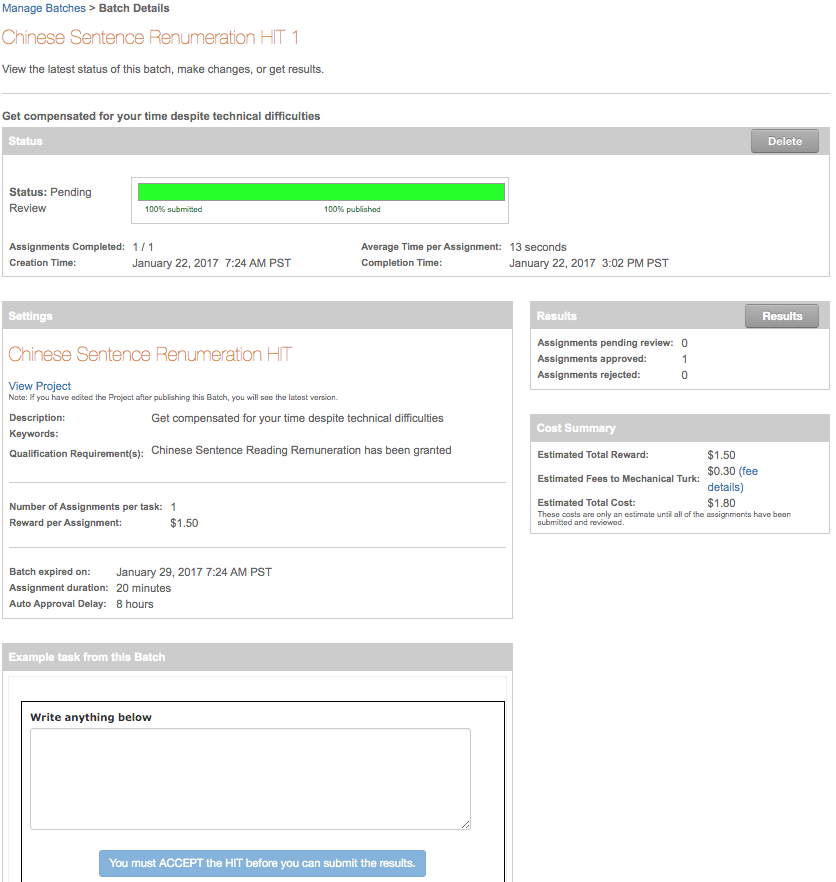
\includegraphics[width=.9\textwidth]{figures/remuneration}
\caption{Screenshot of a HIT made specifically to remunerate workers who could not complete the experiment because of technical difficulties.}
\label{default}
\end{center}
\end{figure}

\subsection{Granting bonuses}

In addition to payments, MTurk provides the option to grant a bonus to a worker. This option can come in handily, for example, when there are multiple visits to an experiment (e.g., a longitudinal study). In that case the reward would be the basic payment that the worker received for completing any part of the experiment, and the bonus would be used as an incentive to complete {\em all} visits of the experiment. *Mturkutils* comes with a separate script to grant bonuses to workers.




\end{document}
